\documentclass[10pt,a4paper]{article}
\usepackage[T1]{fontenc}
\usepackage[utf8]{inputenc}
\usepackage{lmodern}
\usepackage[margin=20mm]{geometry}
\usepackage{amsmath,amssymb,graphicx}
\setlength{\parindent}{0pt}
\setlength{\parskip}{3pt}
\newcounter{reportfigure}
\newcommand{\reportcaption}[1]{\refstepcounter{reportfigure}\par{\small Figure~\thereportfigure: #1\par}}
\setlength{\abovedisplayskip}{6pt}
\setlength{\belowdisplayskip}{6pt}
\newcommand{\answer}[1]{\par\smallskip\textbf{#1}\enspace}
\makeatletter
\def\input@path{{report/}{./}}
\makeatother
\graphicspath{{images/}{report/images/}}
\begin{document}
\begin{center}
{\Large\bfseries Automatic Control III --- Laboratory 2}\\[2pt]
{\normalsize Report: Parts I and II \quad---\quad Mat\'{i}as Garc\'{i}a}
\end{center}
\textbf{Part I: theoretical activity.} Questions 1--3 follow the laboratory guide, pp.~2--3. Results are obtained by numerical simulation; settling time uses a 2\% error band.
\section*{Question 1 --- Inverted pendulum}
\answer{(a) State-space model}
With $x=[\theta,\dot\theta]^\mathsf{T}$, input $u$ and output $y=\theta$,
\begin{equation}
 \dot x_1=x_2,\qquad
 \dot x_2=19.62\sin x_1-x_2+20\cos x_1\,u,\qquad y=x_1.
\end{equation}
The Simulink plant uses two Integrators and the gravity, friction and input terms above. Initial state: $x(0)=[0.1,0]^\mathsf{T}$ (rad, rad/s).

\answer{(b) Input-output linearization and validity}
Differentiating $y$ twice exposes $u$:
\begin{equation}
 \ddot y=19.62\sin\theta-\dot\theta+20\cos\theta\,u.
 \qquad
 \boxed{u=\frac{0.05v-0.981\sin\theta+0.05\dot\theta}{\cos\theta}.}
\end{equation}
Then $\ddot y=v$. The new states remain $z_1=\theta$, $z_2=\dot\theta$, with $\dot z_1=z_2$, $\dot z_2=v$. Relative degree equals the state dimension; there are no internal dynamics. The law requires $\cos\theta\ne0$; around upright its connected domain is $|\theta|<\pi/2$. Required input can grow near the boundary.

\answer{(c) Linear regulation: approximately 1 s settling}
Choose $v=-k_p\theta-k_d\dot\theta$. Matching a repeated pole at $-6$ gives
\begin{equation}
 s^2+k_ds+k_p=(s+6)^2,
 \qquad \boxed{k_p=36,\quad k_d=12.}
\end{equation}
The exact response is $\theta(t)=0.1(1+6t)e^{-6t}$. Thus $(1+6T_s)e^{-6T_s}=0.02$ gives $T_s=0.9723$ s, with no overshoot.

\answer{(d) Closed-loop simulation}
\begin{center}
$\boxed{\text{Linear state feedback}}\xrightarrow{v}
\boxed{\text{Nonlinear cancellation}}\xrightarrow{u}
\boxed{\text{Pendulum}}$\\[2pt]
\small Measured $\theta,\dot\theta$ feed both controllers.
\end{center}
The simple model is \texttt{part1\_pendulum\_regulation.slx}. Run for 2 s using \texttt{ode45}, maximum step 0.005 s, relative/absolute tolerances $10^{-8}/10^{-10}$. The Angle, Rate, Acceleration and Input scopes observe the loop.
\begin{center}
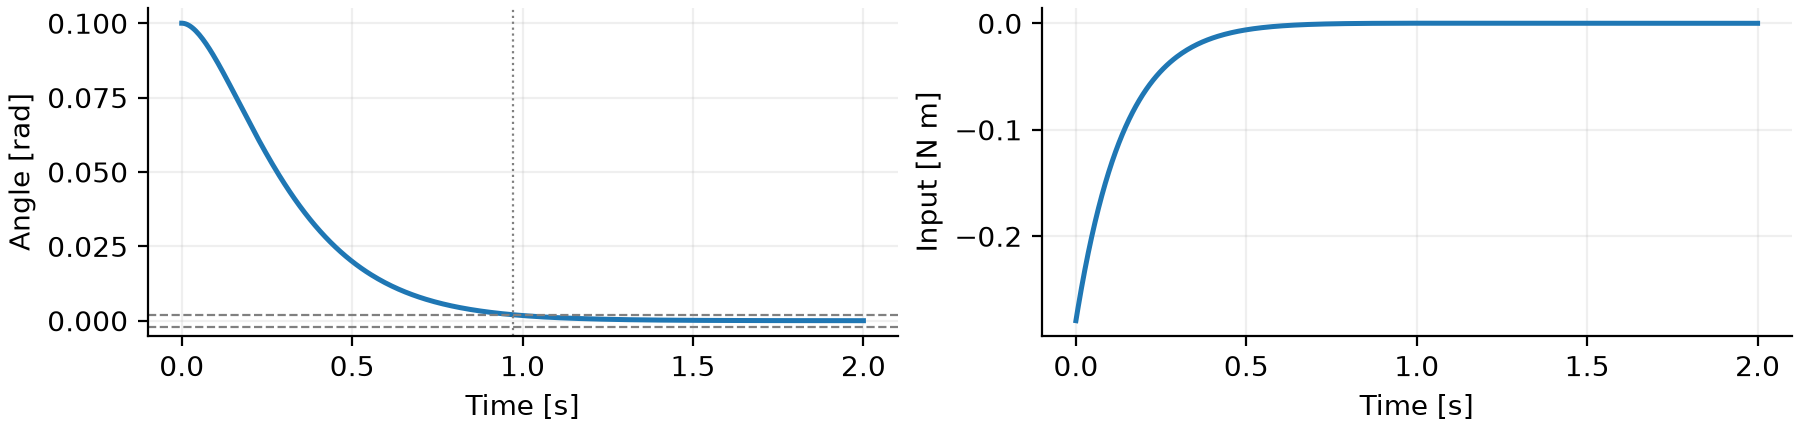
\includegraphics[width=\linewidth]{report_pendulum_response.png}
\reportcaption{Logged simulation signals; the dashed band is $\pm0.002$ rad. The schematic above is explanatory, not a UI screenshot.}
\end{center}
The sampled 2\% settling time is \textbf{0.9762 s}, satisfying the approximate 1 s requirement. Peak $|u|=0.2793$ N\,m. Seven validation cases passed; the largest angle discrepancy from the analytical response was $1.37\times10^{-11}$ rad. These results assume exact cancellation and unconstrained input; no hardware test is claimed.

\clearpage
\section*{Question 2 --- DC motor with quadratic drag}
\answer{(a) State-space model}
Let $x_1=\theta$, $x_2=\omega=\dot\theta$ and $x_3=i_a$, with armature voltage $u$ and output $y=\theta$. Then
\begin{equation}
x=\begin{bmatrix}\theta\\\omega\\i_a\end{bmatrix},\qquad
\boxed{\dot x=
\begin{bmatrix}x_2\\\frac{K_Tx_3-d_1x_2-d_2x_2|x_2|}{J}\\-\frac{K_ex_2+R_ax_3}{L_a}\end{bmatrix}
+\begin{bmatrix}0\\0\\1/L_a\end{bmatrix}u},\qquad
y=\begin{bmatrix}1&0&0\end{bmatrix}x.
\end{equation}
The Simulink plant has three Integrators and separate mechanical/electrical equations; the closed-loop block diagram is shown in Appendix~A.

\answer{(b) Input-output linearization, new states and validity}
Define $\alpha=(K_Ti_a-d_1\omega-d_2\omega|\omega|)/J$ and $D(\omega)=d_1+2d_2|\omega|$. Since $\frac{d}{d\omega}(\omega|\omega|)=2|\omega|$, including at zero,
\begin{equation}
\dot y=\omega,\quad\ddot y=\alpha,\quad
y^{(3)}=-\frac{K_T}{JL_a}(R_ai_a+K_e\omega)-\frac{D(\omega)}{J}\alpha+\frac{K_T}{JL_a}u.
\end{equation}
Thus the linearizing voltage is
\begin{equation}
\boxed{u=R_ai_a+K_e\omega+\frac{L_a}{K_T}\bigl[Jv+D(\omega)\alpha\bigr]}
\quad\Longrightarrow\quad y^{(3)}=v.
\end{equation}
Choose $z=[\theta,\omega,\alpha]^\mathsf{T}$; then $\dot z_1=z_2$, $\dot z_2=z_3$, $\dot z_3=v$. Its inverse is $i_a=(Jz_3+d_1z_2+d_2z_2|z_2|)/K_T$. For $J,L_a,K_T>0$, the input coefficient $K_T/(JL_a)$ and coordinate Jacobian determinant $K_T/J$ never vanish. The law is globally defined for finite ideal-model states, including speed reversal. The transformation is $C^1$; there are no internal dynamics.

\answer{(c) Reference tracking: approximately 0.2 s settling}
For a constant reference $r=\theta_d$, choose
\begin{equation}
v=k_1(r-z_1)-k_2z_2-k_3z_3.
\end{equation}
The error $e=r-\theta$ satisfies $e^{(3)}+k_3\ddot e+k_2\dot e+k_1e=0$. Matching its polynomial to $(s+\lambda)^3$ gives
\begin{equation}
\boxed{k_1=\lambda^3,\qquad k_2=3\lambda^2,\qquad k_3=3\lambda.}
\end{equation}
From rest, $e(t)/e(0)=e^{-\lambda t}[1+\lambda t+(\lambda t)^2/2]$. Choose $\lambda=\tau_\varepsilon/T_s$, where $e^{-\tau_\varepsilon}(1+\tau_\varepsilon+\tau_\varepsilon^2/2)=\varepsilon$. For $\varepsilon=0.02$ and $T_s=0.2$ s, select $\lambda=38$ s$^{-1}$, yielding $k_1=54872$, $k_2=4332$, $k_3=114$ and predicted settling of 0.198 s. For smooth moving references, add $r^{(3)}+k_3\ddot r+k_2\dot r$ to the control law.

\answer{(d) Closed-loop simulation}
For simulation, use $J=0.01$, $K_T=K_e=0.2$, $R_a=2$, $L_a=0.05$, $d_1=0.01$ and $d_2=0.005$ in the supplied SI units. The input coefficient becomes $K_T/(JL_a)=400$. Acceleration is calculated from speed and current. From zero state, the reference steps to 0.1 rad at 0.05 s. The simulation runs for 0.5 s using \texttt{ode45}, maximum step 0.0005 s and relative/absolute tolerances $10^{-8}/10^{-10}$.
\begin{center}
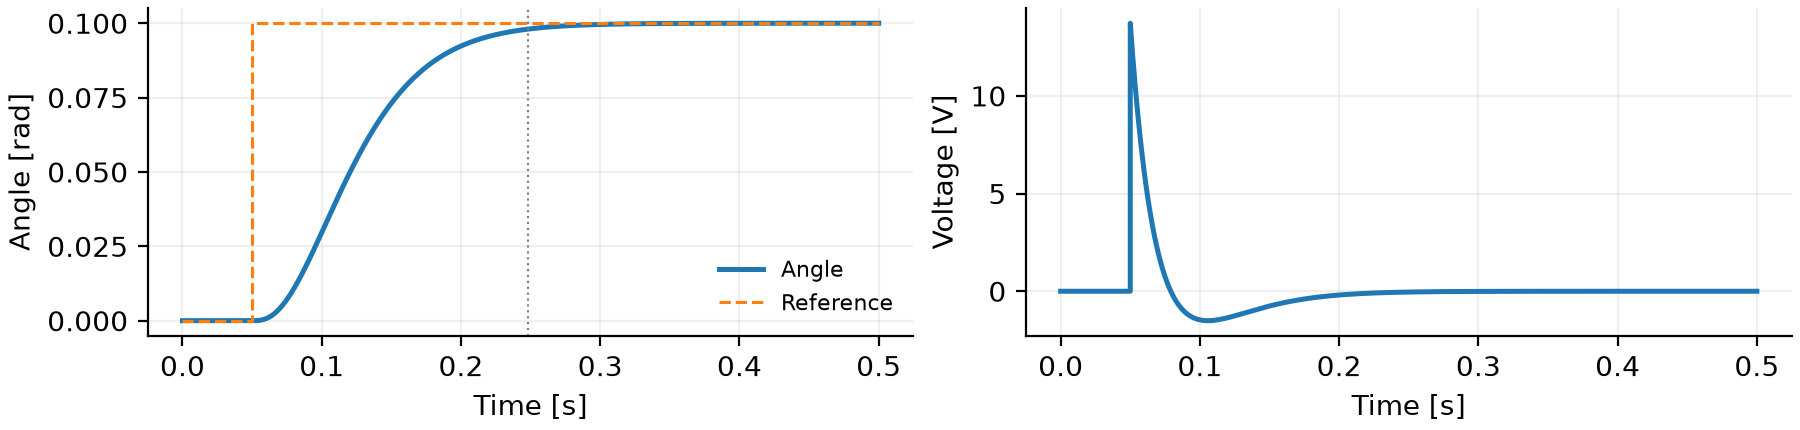
\includegraphics[width=\linewidth]{report_dc_motor_tracking.png}
\reportcaption{Simulated position tracking and applied voltage. Settling time is measured from the reference step.}
\end{center}
The measured 2\% settling time is \textbf{0.198 s}, meeting the approximate 0.2 s requirement, with no overshoot. Peak voltage is 13.718 V for the 0.1 rad step. Six cases check signed references, different initial states, the analytical closed-loop response and the exported model. Larger commands require larger voltage (27.436 V for a 0.2 rad step); no actuator limits or hardware feasibility are assumed.


\clearpage
\section*{Question 3 --- Non-isothermal CSTR}
\answer{(a) State-space model}
Define $\nu=q/V$, $\beta=-\Delta H/(\rho C_p)$, $\gamma=UA/(\rho C_pV)$ and $\kappa(T)=k_0e^{-E/(R_gT)}$, with all rates expressed in seconds. For $x_1=C_A$, $x_2=T$, input $u=T_c$ and output $y=T$,
\begin{equation}
x=\begin{bmatrix}C_A\\T\end{bmatrix},\qquad
\boxed{\dot x=
\begin{bmatrix}\nu(C_{Af}-x_1)-\kappa(x_2)x_1\\\nu(T_f-x_2)+\beta\kappa(x_2)x_1-\gamma x_2\end{bmatrix}
+\begin{bmatrix}0\\\gamma\end{bmatrix}u},\qquad
y=\begin{bmatrix}0&1\end{bmatrix}x.
\end{equation}
The plant integrates concentration and temperature separately (Appendix~A).

\answer{(b) Linearization, validity and zero dynamics}
The input appears after one output derivative:
\begin{equation}
\dot y=\nu(T_f-T)+\beta\kappa(T)C_A+\gamma(u-T).
\end{equation}
Choose
\begin{equation}
\boxed{u=T+\frac{v-\nu(T_f-T)-\beta\kappa(T)C_A}{\gamma}}
\quad\Longrightarrow\quad\dot y=v.
\end{equation}
The new coordinates $z_1=T$, $\eta=C_A$ satisfy
\begin{equation}
\dot z_1=v,\qquad \dot\eta=\nu C_{Af}-[\nu+\kappa(z_1)]\eta.
\end{equation}
The relative degree is $1<2$, leaving one internal state. The coordinate change is an invertible permutation. For $\gamma\ne0$, the law is defined for $T>0$, $C_A\ge0$; practical operation also requires an achievable coolant temperature.

Set the shifted output $T-T_d$ to zero, so that $T\equiv T_d$. The zero dynamics are
\begin{equation}
\dot\eta=\nu C_{Af}-[\nu+\kappa(T_d)]\eta,\quad
\eta^*=\frac{\nu C_{Af}}{\nu+\kappa(T_d)},\quad
\eta(t)=\eta^*+[\eta(0)-\eta^*]e^{-[\nu+\kappa(T_d)]t}.
\end{equation}
For $\nu>0$ and $\kappa(T_d)\ge0$, the internal equilibrium is asymptotically stable; the reactor is minimum phase in this domain.

\answer{(c) Implementation}
The linearizing law receives $C_A$, $T$ and virtual temperature rate $v$, and commands $T_c$. Both states are fed back; the original nonlinear balances are retained.

\answer{(d) Temperature tracking with 5 s settling}
For constant $T_d$, choose $v=\lambda(T_d-T)$. Then $\dot e=-\lambda e$ and $e(t)=e(0)e^{-\lambda t}$, giving
\begin{equation}
\boxed{\lambda=\frac{-\ln\varepsilon}{T_s}},\qquad
\varepsilon=0.02,\ T_s=5\ \mathrm{s}
\quad\Longrightarrow\quad\lambda=0.782405\ \mathrm{s}^{-1}.
\end{equation}
For simulation, $\nu=\gamma=1/60$ s$^{-1}$, $k_0=7.2\times10^{10}/60$ s$^{-1}$, $E/R_g=8750$ K, $\beta=200$ K\,L/mol, $C_{Af}=1$ mol/L and $T_f=350$ K. At $T_d=330$ K, $\eta^*=0.819833$ mol/L and the internal time constant is $[\nu+\kappa(T_d)]^{-1}=49.19$ s. Initially $T=310$ K and $C_A=\nu C_{Af}/[\nu+\kappa(310)]=0.961796$ mol/L. The reference changes to 330 K at 1 s. Simulate 180 s using \texttt{ode45}, maximum step 0.02 s and relative/absolute tolerances $10^{-8}/10^{-10}$.
\begin{center}
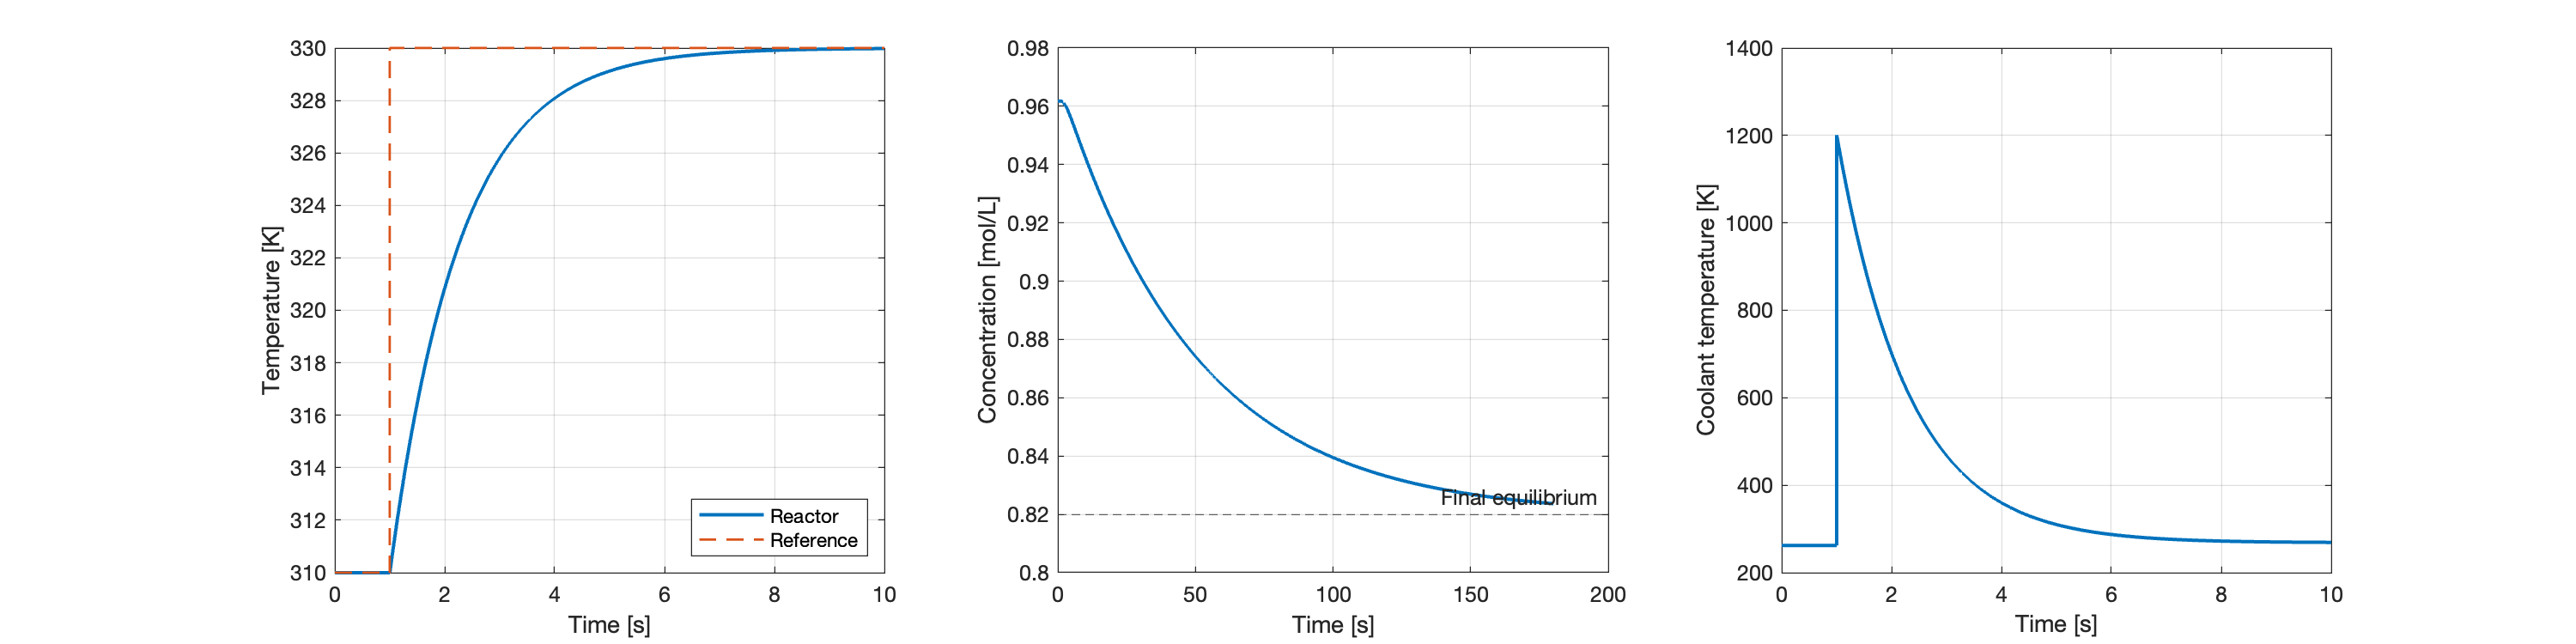
\includegraphics[width=0.95\linewidth]{report_cstr_response.png}
\reportcaption{Simulated temperature tracking, concentration and coolant command. Temperature and concentration use different time scales.}
\end{center}
The temperature follows $T(t)=330-20e^{-\lambda(t-1)}$ K for $t\ge1$ s, without overshoot. The sampled 2\% settling time is \textbf{5.02 s}, consistent with the 5 s target and 0.02 s sampling interval. Concentration reaches 0.82370 mol/L at 180 s and converges toward 0.819833 mol/L; the 5 s requirement applies to temperature only. The initial coolant demand reaches approximately \textbf{1201 K}: the fast transient is achieved mathematically through unconstrained actuation, not within an established coolant operating range.


\par\medskip
\textbf{Part II --- Quanser AERO 2.} To be documented in the next revision.
\end{document}
